% 評価方法

\section{概要}

本章では,本研究で試作した小型 CO$_2$ 測定デバイスを用い,従来の据え置き型 CO$_2$ センサと比較して,同一環境において同様の CO$_2$ 濃度変化が得られるかを評価する。また,測定デバイスを携帯した状態で,様々な環境において問題なく CO$_2$ 濃度を測定できるかを検証する。はじめに,福岡県赤村に設置されているドームハウス内において,従来の据え置き型 CO$_2$ センサを 35 台設置し,それぞれの近傍に本研究で試作した小型 CO$_2$ 測定デバイスを配置した。この環境において両者の測定値を比較し,CO$_2$ 濃度の時間変化が同様の傾向を示すかを確認した。次に,携帯型デバイスとしての有効性を評価するため,測定デバイスを首の前,首の後ろ,腰の前,腰の後ろの計 4 箇所に装着し,赤村周辺の山道を登る測定を行った。この測定では,装着位置や移動によってCO$_2$ 濃度に異常な変動が生じないかを確認した。
以下では,各測定環境および測定方法について詳述する。

\section{測定環境}
  \subsection{赤村ドームハウス}
  本研究で測定対象とした赤村ドームハウスは,福岡県田川郡赤村に位置する多目的利用施設であり,地域活動や宿泊体験,ワークショップ等に利用されている建築物である。本施設は半球状に近いドーム型構造を有しており,内部は天井高が高く,床面から天井付近まで連続した一つの空間として構成されている。ドームハウス内部は,壁面や天井に仕切りが少なく,空気の流れや滞留が空間全体の構造に大きく影響される特徴を持つ。このような構造は,換気条件や人の滞在状況によってCO$_2$ 濃度の空間分布が生じやすいと考えられ,室内空気質の評価を行う測定環境として適している。本測定では,ドームハウス内の高さ方向における CO$_2$ 濃度分布を把握するため,先行研究で使用された据え置き型 CO$_2$ センサを合計 35 台設置した。各センサは,床付近から階段部,2 階部分,および天井付近に至るまで,異なる高さ位置に配置されており,空間全体の CO$_2$ 濃度分布を詳細に取得できる構成とした。

また,各据え置き型 CO$_2$ センサの近傍に,本研究で試作した小型 CO$_2$ 測定デバイスを順次配置し,同一環境・同一高さにおける測定値の比較を行った。これにより,多数の据え置き型センサによる測定結果を基準として,携帯型デバイスによる測定が空間内の換気状態をどの程度把握できるかを評価した。
図\ref{fig:domeHouse}にドームハウスの外観を,図\ref{fig:inside}に内部の様子を示す。
  

\begin{figure}[htbp]
  \centering
  \begin{subfigure}{0.4\linewidth}
    \centering
    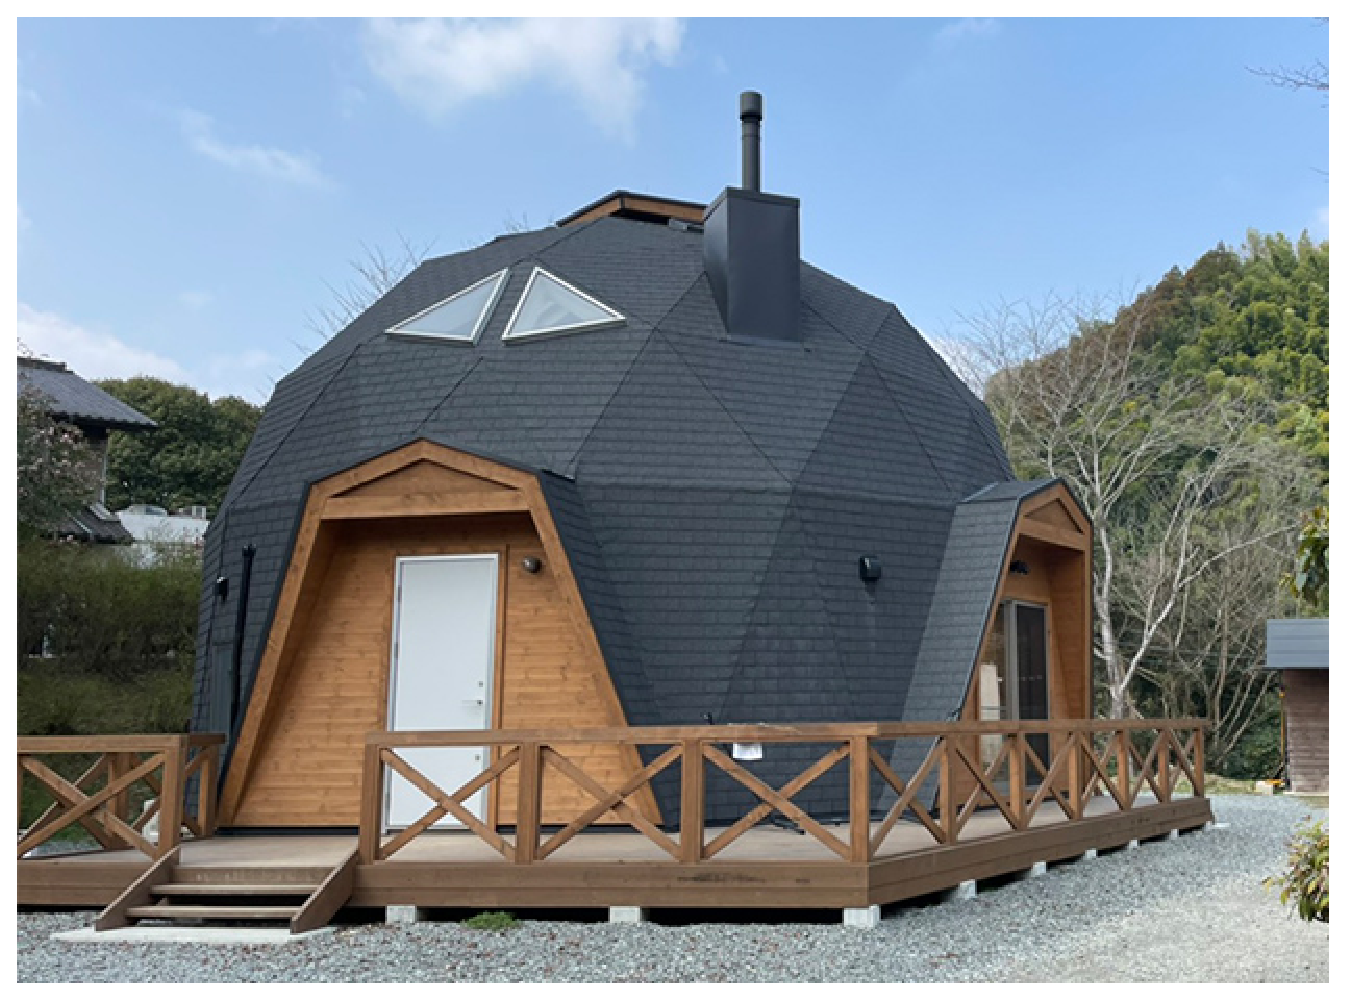
\includegraphics[width=\linewidth]{figures/domeHouse}
    \caption{ドームハウスの外観}
    \label{fig:domeHouse}
  \end{subfigure}
  \hfill
  \begin{subfigure}{0.4\linewidth}
    \centering
    
\includegraphics[width=\linewidth]{figures/inside}
    \caption{ドームハウスの内観}
    \label{fig:inside}
  \end{subfigure}
  \caption{ドームハウスの環境}
  \label{fig:Device1}
\end{figure}

\FloatBarrier


  
  \subsection{山道における携帯測定環境}
山道における携帯測定は,福岡県赤村に位置する岩石山において実施した。岩石山は標高約 454 m の山であり,登山道が整備されたハイキングコースを有している。本測定では,屋外の移動環境において小型 CO$_2$ 測定デバイスを携帯した状態での測定が可能であるかを評価することを目的とした。測定は登山中に実施し,小型 CO$_2$ 測定デバイスを首の前,首の後ろ,腰の前,腰の後ろの計 4 箇所に装着した。これにより,装着位置や身体の動きによってCO$_2$ 濃度の測定値に異常な変動が生じないかを確認した。

\begin{figure}[h]
\centering
\includegraphics[width=.5\linewidth, angle=-90]{./figures/akamurayama}
\caption{山の概要}
\label{fig:akamurayama}
\end{figure}

\begin{figure}[htbp]
  \centering
  \begin{subfigure}{0.45\linewidth}
    \centering
    \includegraphics[width=\linewidth, angle=-90]{figures/collar}
    \caption{首の前}
  \end{subfigure}
  \hfill
  \begin{subfigure}{0.45\linewidth}
    \centering
    \includegraphics[width=\linewidth, angle=-90]{figures/collar}
    \caption{首の後ろ}
  \end{subfigure}

  \vspace{3mm}

  \begin{subfigure}{0.45\linewidth}
    \centering
    \includegraphics[width=\linewidth, angle=-90]{figures/kosimae}
    \caption{腰の前}
  \end{subfigure}
  \hfill
  \begin{subfigure}{0.45\linewidth}
    \centering
    \includegraphics[width=\linewidth, angle=-90]{figures/kosiusiro}
    \caption{腰の後ろ}
  \end{subfigure}

  \caption{〇〇の様子}
  \label{fig:four_photos}
\end{figure}

\FloatBarrier


\section{測定方法}

\subsection{ドームハウスにおける測定方法}

ドームハウス内における CO$_2$ 濃度分布および換気状態を把握するため,据え置き型 CO$_2$ 測定器と,本研究で試作した小型 CO$_2$ 測定デバイスを用いた測定を行った。本測定では,ドームハウス内部の高さ方向に着目し,床付近から天井付近にかけて CO$_2$ 濃度がどのように変化するかを評価することを目的とした。はじめに,先行研究で使用された据え置き型 CO$_2$ 測定器を用いて測定を行った。据え置き型測定器は合計 35 台使用し,螺旋階段および 2 階部分に設置された棚を含め,床面付近から天井付近までの高さ方向に配置した。各測定器には EXAKA1 から EXAKA35 の識別子を付与し,EXAKA1 を最下部,EXAKA35 を最上部とした。測定は同一時間帯に実施し,各測定器から得られた CO$_2$ 濃度データを用いて,ドームハウス内における高さ方向の CO$_2$ 濃度分布を把握した。

次に,据え置き型測定器による測定結果を基準として,本研究で試作した小型 CO$_2$ 測定デバイスによる測定を行った。本測定では,多数のセンサを同時に設置する方法ではなく,利用者が携帯型デバイスを用いて任意の位置で測定を行う状況を想定し,小型 CO$_2$ 測定デバイスを携帯した状態で,ドームハウス内の異なる高さ位置において逐次的に CO$_2$ 濃度を測定した。比較測定の手順として,小型 CO$_2$ 測定デバイスを各据え置き型測定器の直近に配置し,同一高さ・同一空間における CO$_2$ 濃度を測定した。測定終了後,小型測定デバイスを一段上の設置位置へ移動させ,同様の測定を繰り返した。この操作を EXAKA1 から EXAKA35 までの全ての据え置き型測定器に対して順に実施し,合計 35 箇所における比較測定を行った。
測定時には,小型 CO$_2$ 測定デバイスと据え置き型 CO$_2$ 測定器が可能な限り近接するよう配置し,同一高さ・同一環境条件における CO$_2$ 濃度を測定できるよう配慮した。小型測定デバイスによる測定は,各高さ位置において測定ボタンを操作することで実施した。

\begin{figure}[htbp]
  \centering
  \begin{subfigure}{0.45\linewidth}
    \centering
    \includegraphics[width=\linewidth,angle=-90]{figures/akamurakaidan}
    \caption{階段}
    \label{fig:Device0}
  \end{subfigure}
  \hfill
  \begin{subfigure}{0.45\linewidth}
    \centering
    \includegraphics[width=\linewidth]{figures/akamura2kai}
    \caption{階段の上部}
    \label{fig:Finishing machine}
  \end{subfigure}
  \caption{プロトタイプおよび測定機器1の外観}
  \label{fig:Device1}
\end{figure}

\FloatBarrier


  \subsection{携帯時の測定方法}

携帯時の測定では,小型 CO$_2$ 測定デバイスを利用者の身体に装着し,登山中に連続して CO$_2$ 濃度を測定した。装着位置は,首の前,首の後ろ,腰の前,腰の後ろの計 4 箇所とした。測定中は通常の歩行動作を行い,移動や姿勢変化によって測定値に大きな変動や異常値が発生しないかを確認した。

\section{測定条件}
\subsection{測定間隔}

山道における測定では,スマートフォンのテザリング接続が一定時間通信を行わない場合に切断される特性を考慮し,測定間隔を 30 秒とした。これにより,通信が途切れることなく安定して測定データを取得できるようにした。ドームハウスでの測定では,各測定位置において小型 CO$_2$ 測定デバイスを据え置き型測定器の近傍に設置して測定を行い,測定終了後は速やかに次の測定位置へ移動した。

\subsection{装着位置}
装着位置は,日常的な携帯を想定し,首および腰の前後の 4 箇所とした。

\subsection{測定時間}

ドームハウスにおける測定では,最下部に設置された測定器から最上部に設置された測定器までの全測定位置において比較測定を行い,測定全体に要した時間は約 30 分間であった。山道における測定では,登山開始から登頂および下山完了までの約 2 時間にわたり測定を行った。

\section{評価方法}
  \subsection{CO$_2$ 濃度測定精度の評価方法}

CO$_2$ 濃度測定精度の評価は,据え置き型 CO$_2$ 測定器を基準として,本研究で試作した小型 CO$_2$ 測定デバイスの測定結果を比較することで行った。評価では,測定値の絶対値の一致ではなく,時間変化の傾向が一致しているかに着目した。具体的には,同一位置・同一環境において取得した据え置き型測定器および小型測定デバイスのCO$_2$ 濃度の時間変化を比較し,両者が同様の増減傾向を示す場合に,測定精度が十分であると判断した。

  
   \subsection{省電力性能の評価方法}

省電力性能の評価は,ドームハウスおよび山道での測定とは別に,教室内において実施した。本評価では,測定機器を通常の測定動作状態で動作させ,バッテリ駆動時における連続稼働時間を確認した。評価時の測定条件として,測定間隔は 5 分とし,測定時以外の時間は ESP32-C6 を DeepSleep 状態へ移行させた。測定機器は,バッテリ電圧の低下により動作が停止するまで連続動作させ,その動作時間を稼働時間として記録した。本研究では,測定機器からサーバへ送信された測定データの確認および評価を行うため,研究室内で開発された iOS アプリを使用した。本アプリは,サーバにアップロードされた CO$_2$ 濃度データを時系列グラフとして表示する機能を備えており,測定中の動作確認および測定終了時刻の判断に利用した。

